% !TeX root = ../main.tex
% Add the above to each chapter to make compiling the PDF easier in some editors.

\chapter{Comparison}\label{chapter:04_comparison}

In this section we are going to analyse the results of the first 15 testcases we got from the SteinerLib. We are going to constrast the solutions from the respective approximation with the optimal solution cost, which is referenced in the testcase database \cite{Dui93}. We are also going to look at the solution tree of testcase 41, its solution for the three algorithms differs substantially enough to nicely showcase their different approaches. The trees were output as a .dot file and visualized using the open source software "graphviz". 

\section{MST approximation}

\begin{figure}[htbp]
\centering
\includegraphics[scale=0.15]{figures/MST.png}
\caption{Output tree of the MST-approximation algorithm for Graph 41}\label{fig:MSTTree41}
\end{figure}

\begin{table}[htbp]
 \caption{Results of MST for 15 testcases from SteinerLib \cite{Dui93}}\label{tab:MSTResults} 	
 \centering
 \begin{tabular}{l l l l}
\toprule
Graph & Opt & MST & MST-Opt \\
\midrule
11	& 1479	& 1585		& 106 \\
12	& 1484	& 1788		& 304 \\
13	& 1381	& 1676		& 295 \\
14	& 1397	& 1679		& 280 \\
15	& 1495	& 1602		& 107 \\
\midrule 
21	& 1175	& 1471		& 296 \\
22	& 1178	& 1477		& 299 \\
23	& 1174	& 1471		& 297 \\
24	& 1161	& 1473	 	& 312 \\
25	& 1162	& 1483		& 321 \\
\midrule
41	& 1276	& 1600		& 324 \\
42	& 1287	& 1674		& 387 \\
43	& 1295	& 1689		& 394 \\
44	& 1366	& 1676		& 310 \\
45	& 1310	& 1751		& 441 \\
\bottomrule
\end{tabular}
\end{table}


\section{Berman and Ramaiyer}

\begin{table}[htbp]
 \caption{Results of Berman, Ramaiyer for 15 testcases from SteinerLib \cite{Dui93}}\label{tab:BeRaResults} 	
 \centering
 \begin{tabular}{l l l l l}
\toprule
Graph & Opt & BeRa & BeRa\% & BeRa-Opt \\
\midrule
11	& 1479	& 1585	& 1.072	& 106 \\
12	& 1484	& 1788	& 1.205	& 304 \\
13	& 1381	& 1676	& 1.214	& 295 \\
14	& 1397	& 1679	& 1.202	& 282 \\
15	& 1495	& 1602	& 1.072	& 107 \\
\midrule 
21	& 1175	& 1471	& 1.252	& 296 \\
22	& 1178	& 1477	& 1.254	& 299 \\
23	& 1174	& 1471	& 1.253	& 297 \\
24	& 1161	& 1473	& 1.269 	& 312 \\
25	& 1162	& 1483	& 1.276	& 321 \\
\midrule
41	& 1276	& 1578	& 1.234	& 302 \\
42	& 1287	& 1658	& 1.288	& 371 \\
43	& 1295	& 1689	& 1.304	& 394 \\
44	& 1366	& 1676	& 1.227	& 310 \\
45	& 1310	& 1751	& 1.337	& 441 \\
\bottomrule
\end{tabular}
\end{table}

\begin{figure}[htbp]
\centering
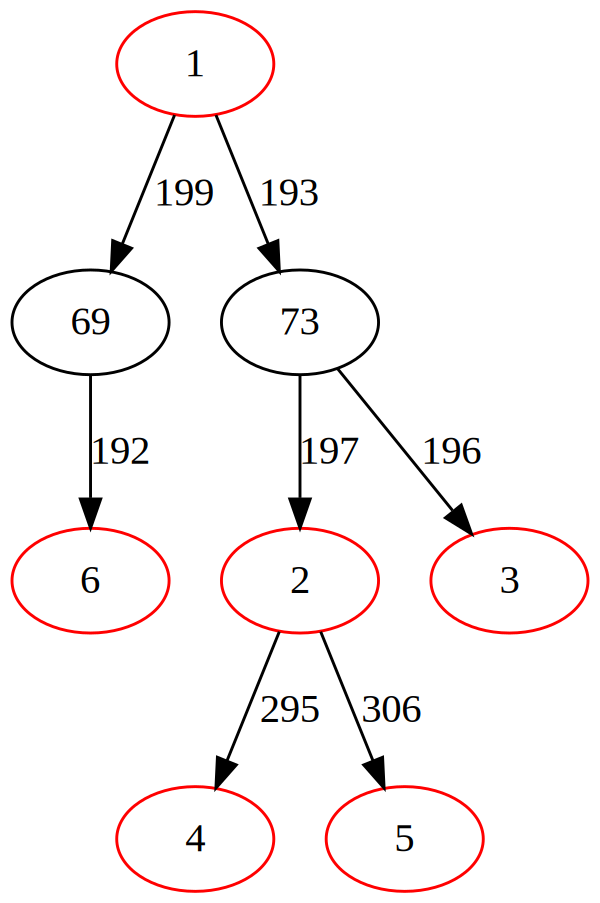
\includegraphics[scale=0.25]{figures/BermanRamaiyer.png}
\caption{Output tree of the Berman, Ramaiyer algorithm for Graph 41}\label{fig:BeRaTree41}
\end{figure}

\section{Hougardy and Proemel}

\begin{table}[htbp]
 \caption{Results of $IRGH$ for 15 testcases from SteinerLib \cite{Dui93}}\label{tab:HoPrResults} 	
 \centering
 \begin{tabular}{l l l l l}
\toprule
Graph & Opt & HoPr & HoPr\% & HoPr-Opt \\
\midrule
11	& 1479	& 1654	& 1.118	& 175 \\
12	& 1484	& 1759	& 1.185	& 275 \\
13	& 1381	& 1471	& 1.065	& 90 \\
14	& 1397	& 1848	& 1.323	& 451 \\
15	& 1495	& 1895	& 1.268	& 400 \\
\midrule 
21	& 1175	& 1471	& 1.252	& 296 \\
22	& 1178	& 1477	& 1.254	& 299 \\
23	& 1174	& 1471	& 1.253	& 297 \\
24	& 1161	& 1473	& 1.269 	& 312 \\
25	& 1162	& 1483	& 1.276	& 321 \\
\midrule
41	& 1276	& 1463	& 1.147	& 187 \\
42	& 1287	& 1631	& 1.267	& 344 \\
43	& 1295	& 1535	& 1.185	& 240 \\
44	& 1366	& 1546	& 1.132	& 180 \\
45	& 1310	& 1616	& 1.234	& 306 \\
\bottomrule
\end{tabular}
\end{table}

\begin{figure}[htbp]
\centering
\includegraphics[scale=0.40]{figures/HougardyProemel.png}
\caption{Output tree of the $IRGH$-approximation algorithm for Graph 41}\label{fig:HoPrTree41}
\end{figure}
